% =================================================================================================
% File:			all.tex
% Description:	Defiinisce la sezione relativa a ...
% Created:		2015-01-29
% Author:		Tesser Paolo
% Email:		p.tesser921@gmail.com
% =================================================================================================
% Modification History:
% Version		Modifier Date		Change												Author
% 0.0.1 		2015-01-29 			iniziata stesura documento di prova					Tesser Paolo
% =================================================================================================
% 0.0.2			2015-02-02			aggiunta img + migliorata sez. configurazioni		Tesser Paolo
% =================================================================================================
% 0.0.3			2015-02-02			aggiunta sezione per i workflow, da stendere		Tesser Paolo
% =================================================================================================
% 0.0.4			2015-02-03			commentate due parti di codice (verbatim) per bug	Tesser Paolo
% =================================================================================================
% 0.0.5			2015-02-03			aggiunto comando line 21 per fix bug (solo su git)	Tesser Paolo
% =================================================================================================
% 0.0.6			2015-02-03			stesura sezione sui tips per velocizzare lavoro		Tesser Paolo
% =================================================================================================
% 0.0.7			2015-02-03			sezione branch + commit amend						Tesser Paolo
% =================================================================================================
% 0.0.8			2015-02-04			parte sul merge e sul rebase						Tesser Paolo
% =================================================================================================
%


\global\let\tikz@ensure@dollar@catcode=\relax % fix verbatim PROBLEM

% CONTENUTO DEL CAPITOLO

\section{Introduzione} % (fold)
\label{sec:introduzione}
Git è un sistema di controllo di versione distribuito.
\newline
\textbf{Distribuito} (DVCS) significa che ogni componente, del gruppo di lavoro, possiede una copia locale completa del repository.
\newline

\noindent
\textbf{Vantaggi}:
	\begin{itemize}
		\item operazioni di commit più veloci da effettuare;
		\item si riesce a lavorare offline;
		\item ognuno ha in locale un backup del repository.
	\end{itemize}
	\noindent
	\newline
La seguente immagine serve per dare un idea generale di come git lavori e tramite quali operazioni di base. Viene mostrato inoltre il rapporto tra la gestione in locale del repository con quello in remoto. Il dettaglio delle operazioni sarà illustrato prevalentemente nella sezione \ref{sec:lavorare_sul_repository}.

	\begin{figure}[htbp]
		\centering
		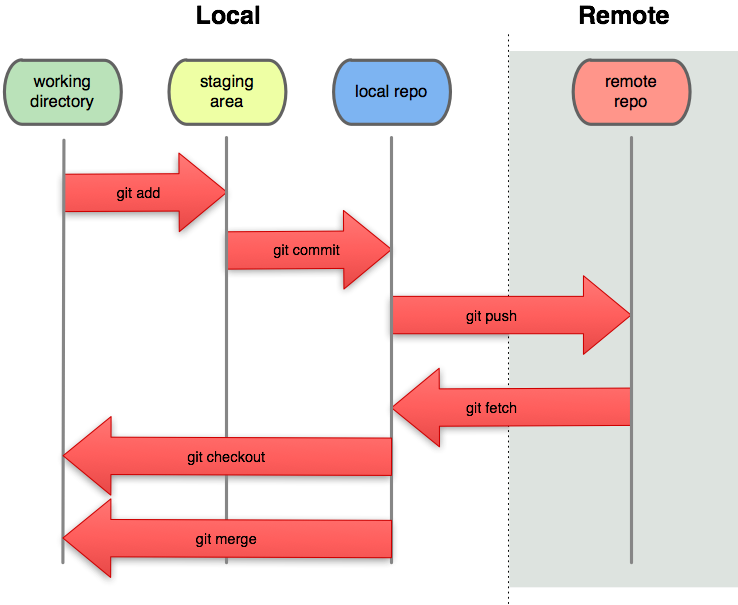
\includegraphics[scale=1.1]{images/git_local_remote.png}
		\caption{Git - Locale e Remoto}
		\label{fig:git_locale_e_remoto}
	\end{figure}


	\subsection{Informativi} % (fold)
	\label{sub:informativi}
		\begin{itemize}
			\item \textbf{CodeSchool}: \url{www.codeschool.com};
			\item \textbf{CERN - Best Practice}: PDF;
		\end{itemize}
	% subsection informativi (end)

% section introduzione (end)

\newpage \clearpage
\section{Riferimenti} % (fold)
\label{sec:riferimenti}
Di seguito viene spiegato attraverso quali nomi git si riferisce a determinati stati del versionamento. \newline \newline

\textbf{Riferimenti specifici}:
	\begin{itemize}
		\item \textbf{Working Tree}: è l'insieme di file su cui si sta lavorando non ancora aggiunti alla staging area (vedi sezione \ref{sub:lavorare_in_locale});
		\item \textbf{Index}: è il riferimento ai file pronti per essere committati, quelli aggiunti alla staging area;
		\item \textbf{HEAD}: è il riferimento all'ultimo commit effettuato;
		\item \textbf{d3a7c852d2c789f791b11091894cc71387e562e9}: un valore hash attribuito ad ogni commit;
		\item \textbf{master, feature-eg}: il nome esatto di un branch per riferirsi ad esso;
		\item \textbf{v1.0.0}: il nome di un tag per riferirsi ad esso.
	\end{itemize}
	\noindent
\textbf{Riferimenti relativi}: TO DO
\begin{comment}
	\begin{itemize}
		\item il commit precedente: ref\textasciitilde1 oppure ref^;
		\item il penultimo commit: ref\textasciitilde2 oppure ref^^;
		\item genitori differenti: ref^1. (TO LEARN).
	\end{itemize}
\end{comment}

% section riferimenti (end)


\newpage \clearpage
\section{Impostare git} % (fold)
\label{sec:impostare_git}
La prima volta che si installa git è buona pratica impostare da subito alcune credenziali. \newline
Queste credenziali possono essere impostate su diversi livelli:
	\begin{itemize}
		\item \textbf{global}: valide quindi per tutti i repository dell'utente. Si trovano nel file:
			\begin{center}
				~/.gitconfig
			\end{center}
		\item \textbf{system}: valide per tutti i repository del computer. Si trovano nel file:
			\begin{center}
				/etc/gitconfig
			\end{center}
		\item \textbf{local}: valide solo per il repository dal quale vengono impostate. Si trovano nel file:
			\begin{center}
				.git/config
			\end{center}
	\end{itemize}
Da linea di comando eseguire i seguenti comandi, cambiando l'opzione ``global'' a seconda delle esigenze:
	\begin{verbatim}
	path: git config --global user.name "Nome Cognome"
	path: git config --global user.email mail@mail.com
	path: git config --global color.ui true
	path: git config --global core.editor emacs
	path: git config --global commit.template ~/.gitmessage.txt
	\end{verbatim}

% section impostare_git (end)

\newpage \clearpage
\section{Creare un repository} % (fold)
\label{sec:creare_un_repository}
Un repository può essere creato in locale e usato solo nel computer dell'utente, anche se questo non permetterà un lavoro collaborativo, oppure, dopo la creazione in locale, può essere associato ad un repository creato su un server (o attraverso un servizio di hosting). \newline
Per creare un repository su un servizio di hosting basta seguire le istruzione che il sito propone.
	\subsection{Creazione in locale} % (fold)
	\label{sub:creazione_in_locale}
	Di seguito viene illustrata la sequenza di comandi che dovranno essere eseguiti:
		\begin{verbatim}
		path: mkdir nome_repo
		path: cd nome_repo
		path: git init
		\end{verbatim}
	\noindent
	L'ultima istruzione creerà tutti i metadati necessari al repository. Verranno salvati nella cartella nascosta:
		\begin{center}
			nome\_repo/.git/
		\end{center}

	% subsection creazione_in_locale (end)

% section creare_un_repository (end)

\newpage \clearpage
\section{Lavorare sul repository} % (fold)
\label{sec:lavorare_sul_repository}

	\subsection{Lavorare in locale} % (fold)
	\label{sub:lavorare_in_locale}
	Le tre azioni che vengono più spesso eseguite quando si lavora in locale sono:
		\begin{itemize}
			\item creare un file;
			\item aggiungerlo alla \textbf{staging area} attraverso il comando:
				\begin{verbatim}
				path: git add <nome_del_file.ext>
				\end{verbatim}
				\noindent
				La staging area è il luogo dove sono presenti i file pronti per essere committati.
				Se si vogliono aggiungere più file contemporaneamente o solo alcuni, possiamo eseguire in esclusione questi comandi:
					\begin{verbatim}
					# aggiunge tutti i file presenti nella unstaging area
					path: git add --all
					path: git add <list of file>
					path: git add *.ext
					path: git add dir/
					\end{verbatim}
				\noindent
				\textbf{Buona pratica}, come verrà illustrato di seguito, vuole che i commit siano il più possibile atomici. \'E \textbf{consigliato fortemente} quindi eseguire il comando:
					\begin{verbatim}
					path: git add --patch (o -p)
					\end{verbatim}
				\noindent
				Questo comando permettere di revisionare il codice che si sta aggiungendo, con la possibilità di scartarne delle parti;

			\item committare i cambiamenti attraverso il comando:
				\begin{verbatim}
				path: git commit -m "msg"
				\end{verbatim}
				\noindent
				Quest'ultima operazione può essere effettuata anche senza l'opzione -m, in tal caso la procedura seguirà lo schema illustrato nella sezione TO DO; \newline
				Importante e \textbf{obbligatorio} è effettuare commit atomici in quanto se qualcosa andasse storto, per colpa di qualche inserimento sbagliato, sarebbe più facile effettuare una ricerca dell'errore. Inoltre, questa metodologia, permette di dare una descrizione più efficace sul messaggio di cosa si sta facendo e soprattutto meno prolissa in quanto vado ad aggiungere meno cose contemporaneamente. \newline
				Il messaggio che viene inserito deve essere di facile interpretazione. Non bisogna scrivere cose generiche o superflue. \newline
				Se ci si accorge di aver dimenticato qualcosa nell'ultimo commit, è sempre possibile, tramite il comando:
				\begin{verbatim}
				path: git commit --amend
				\end{verbatim}
				combinare i file presenti nella staging area con quelli del precedente commit ed estendere il precedente messaggio. Può però anche solo essere usato appunto per cambiare il messaggio, senza aggiungere nulla.\newline
				Questa operazione andrebbe \textbf{esclusivamente} fatta quando non si ha ancora pushato nel repository remoto (pubblico) il cambiamento, altrimenti potrebbe generare qualche conflitto inaspettato (nulla che git non risolva da solo nella maggior parte delle volte). Questo avviene perché l'operazione non altera il commit precedente, ma lo rimpiazza completamente.

		\end{itemize}
	\noindent
	Per osservare i cambiamenti avvenuti dall'ultima operazione di commit basta lanciare il comando:
		\begin{verbatim}
		path: git status
		\end{verbatim}

	
		\subsubsection{Visualizzare le differenze} % (fold)
		\label{ssub:visualizzare_le_differenze}
		Per osservare le differenze di un file in relazione a dove si trova:
		% \begin{comment}
			\begin{verbatim}
			# per osservare le modifiche sui file non ancora inseriti
			# nella staging area con quelli presenti su Index
			path: git diff <nome_del_file>
			# per osservare le modifiche sui file già inseriti nella staging area
			# con quelli presenti su HEAD
			path: git diff --staged <nome_del_file>
			# per osservare le modifiche sui file nella staging area
			# rispetto a quelli su HEAD
			path: git diff HEAD
			\end{verbatim}
		% \end{comment}

		% subsubsection visualizzare_le_differenze (end)



		\subsubsection{Gestione dei cambiamenti} % (fold)
		\label{ssub:gestione_dei_cambiamenti}
		
			\paragraph{Checkout} % (fold)
			\label{par:checkout}
			Per riportare i file che si sono presenti nel working tree, ad un determinato stato, bisogna eseguire il seguente comando:
			\begin{verbatim}
			path: git checkout <commit_ref> <nome_file>
			\end{verbatim}
			Questo mette il puntatore in uno stato diverso da HEAD. Grazie a ciò è impossibile danneggiare il repository mentre si guarda una versione precedente, proprio perché lo stato corrente rimane intoccato. Qualora si volesse utilizzare la versione in cui ci si è spostati, per aggiornare il repository a quello stato, basterebbe ri-committare lo stato in cui siamo e verrebbe creato un nuovo snapshot facendo avanzare l'HEAD.
			% paragraph checkout (end)

			\paragraph{Revert} % (fold)
			\label{par:revert}
			Se vogliamo tornare a una precedente configurazione, \textbf{ma senza cancellare la precedente storia}, dobbiamo utilizzare il seguente comando:
			\begin{verbatim}
			path: git revert <commit_ref>
			\end{verbatim}
			Questo viene fatto appendendo un nuovo commit, avente i file alla versione espressa nel comando. \newline
			\'E \textbf{buona pratica} utilizzare questo comando, a discapito di altri che possono attuare la stessa pratica, quando bisogna agire su un repository pubblico, condiviso con altri.
			% paragraph revert (end)
		
			\paragraph{Reset} % (fold)
			\label{par:reset}
			Per rimuovere dei file aggiunti nella staging area, tramite il comando \textbf{git add}, bisogna lanciare il seguente comando:
				\begin{verbatim}
				path: git reset HEAD # per rimuovere tutti i file
				path: git reset HEAD <nome_del_file> # per rimuovere solo quello specificato
				\end{verbatim}
			\noindent
			La variabile Index viene portata indietro di un passo. \newline \newline
			Per annullare l'ultimo commit dobbiamo eseguire il seguente comando:
				\begin{verbatim}
				path: git reset --soft HEAD^
				\end{verbatim}
			\noindent
			L'opzione \textbf{--soft} serve a lasciare i file, dell'ultima commit, nella staging area, quindi puntati dalla variabile Index. \newline
			La direttiva \textbf{HEAD\^} serve per annullare i commit solo fino al penultimo, cioè quello precedente di quello che vogliano annullare. \newline
			La variabile HEAD viene portata indietro di un passo. \newline
			\textbf{Nota}: questi comandi non annullano le modifiche effettuate ai file. \newline \newline
			Per rimuovere l'ultimo commit dobbiamo eseguire il seguente comando:
				\begin{verbatim}
				path: git reset --hard HEAD^
				\end{verbatim}
			\noindent
			Le variabili HEAD, Index e Working Tree vengono portate indietro di un passo. \newline
			Questo comando è potenzialmente dannoso perché rischi di farti perdere il lavoro presente nella Working Tree. \'E bene quindi utilizzarlo solo quando il comando \textbf{git status} da un output pulito. \newline
			\textbf{Non bisogna} inoltre usare questo comando quando il commit è stato pushato in un repository pubblico, perché altri sviluppatori potrebbero fare riferimento ad un istanza che verrebbe rimossa.
			% paragraph reset (end)
			
		% subsubsection gestione_dei_cambiamenti (end)
		
		
		\subsubsection{Gestione dei branch} % (fold)
		\label{ssub:gestione_dei_branch_locale}
		A differenza di altri sistemi di versionamento, in git un branch è semplicemente un puntatore a un commit. \newline
		Le operazioni di branching sono elencate di seguito:
			\begin{itemize}
				\item creare un branch:
					\begin{verbatim}
					path: git branch <nome_del_branch> [<punto di partenza>]
					\end{verbatim}
				\item cancellare un branch:
					\begin{verbatim}
					path: git branch -d|-D <nome_del_branch>
					\end{verbatim}
				\item muoversi tra i diversi branch:
					\begin{verbatim}
					path: git checkout <nome_del_branch_dove_spostarsi>
					\end{verbatim}
				Questo comando può essere eseguito solo quando non ci sono file ancora da committare;
				\item creare e spostarsi nel branch appena generato:
					\begin{verbatim}
					path: git checkout -b <nome_del_branch>
					\end{verbatim}
				\item rinominare un branch:
					\begin{verbatim}
					path: git branch -m <nome_del_branch_vecchio> <nome_del_branch_nuovo>
					\end{verbatim}
			\end{itemize}
			\noindent
		
		In git ci sono due modi per integrare i cambiamenti di un branch su un altro.
			\begin{enumerate}
				\item \textbf{Rebase e Merge}: eseguendo prima l'operazione di rebase rispetto a quella di merge, sarà permesso muovere un branch da uno snapshot (iniziale) ad un altro, come illustrato nella figura seguente.
					\begin{figure}[htbp]
						\centering
						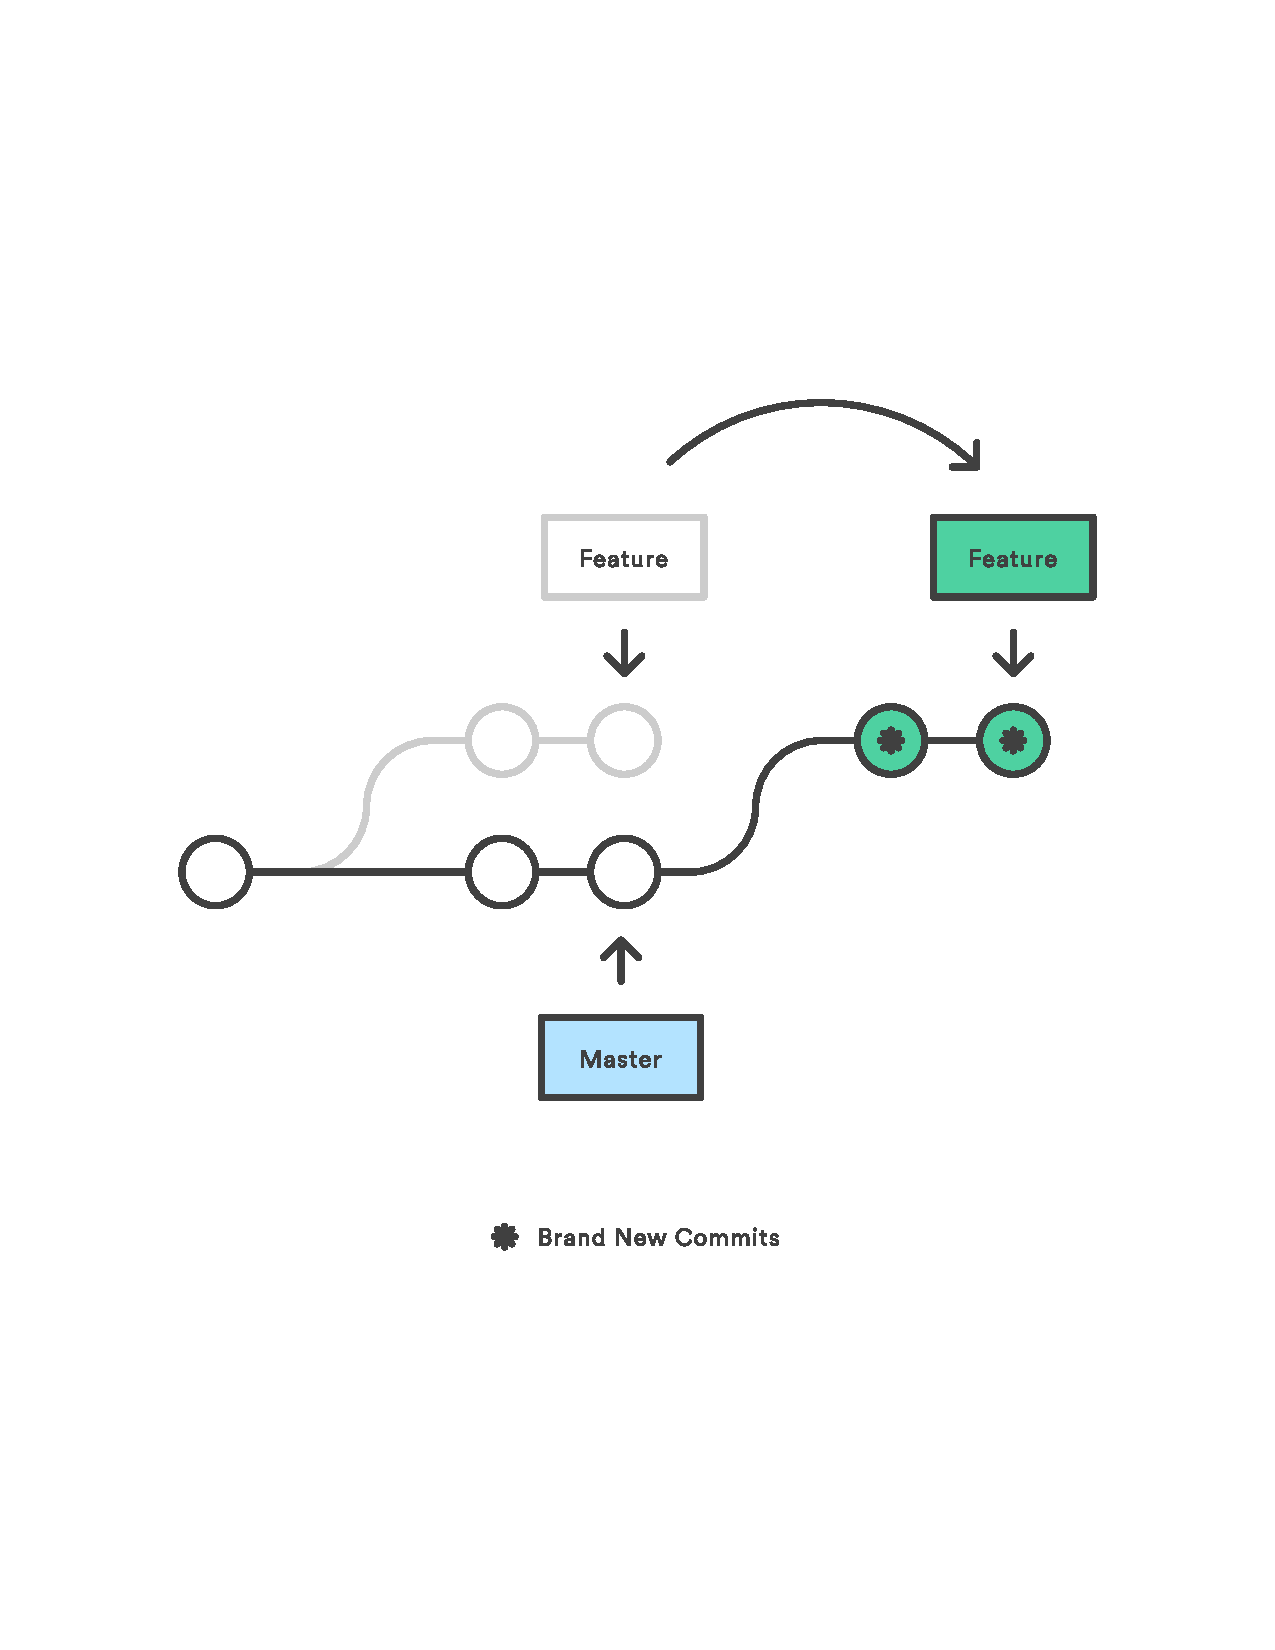
\includegraphics[scale=0.6]{images/rebase.pdf}
						\caption{Git - Rebase a branch}
						\label{fig:git_rebase_a_branch}
					\end{figure}
				

				\item \textbf{Merge}: TO DO.

			\end{enumerate}
		% subsubsection branch (end)


		\subsubsection{Gestione dei tag} % (fold)
		\label{ssub:gestione_dei_tag_locale}
		TO DO
		% subsubsection tag (end)

	% subsection lavorare_in_locale (end)

	\subsection{Lavorare in remoto} % (fold)
	\label{sub:lavorare_in_remoto}
	TO DO
		\subsubsection{Gestione dei branch} % (fold)
		\label{ssub:gestione_dei_branch_remoto}
		Le operazioni di branching sono elencate di seguito:
			\begin{itemize}
				\item TO DO
			\end{itemize}
		% subsubsection gestione_dei_branch (end)

		\subsubsection{Gestione dei tag} % (fold)
		\label{ssub:gestione_dei_tag_remoto}
		TO DO
		% subsubsection gestione_dei_tag (end)

	% subsection lavorare_in_remoto (end)

% section lavorare_sul_repository (end)

\newpage \clearpage
\section{Tips per velocizzare il lavoro} % (fold)
\label{sec:tips_per_velocizzare_il_lavoro}
Esistono diversi modi per velocizzare l'uso di git, in modo da renderlo meno frustrante e più appetibile durante le attività di sviluppo.
	\subsection{Auto completamento} % (fold)
	\label{sub:auto_completamento}
	Git di base non offre l'auto completamento per i suoi comandi, bisogna ogni volta quindi scriverli per esteso. Seguendo le istruzioni presenti al seguente link: \url{http://code-worrier.com/blog/autocomplete-git/} sarà possibile abilitare questa funzionalità.
	% subsection auto_completamento (end)

	\subsection{Alias} % (fold)
	\label{sub:alias}
	Un altro modo più veloce di eseguire i comandi di git, è definendo degli alias per i comandi che utilizziamo maggiormente. Questo può essere fatto nel modo seguente:
	\begin{verbatim}
		# comandi singoli
		path: git config --gloabl alias.nome_alias nome_comando
		# comandi con opzioni
		path: git config --gloabl alias.nome_alias 'nome_comando opzione'
	\end{verbatim}
	% subsection alias (end)

% section tips_per_velocizzare_il_lavoro (end)

\newpage \clearpage
\section{Git Hooks} % (fold)
\label{sec:git_hooks}
TO DO


% section git_hooks (end)




\newpage \clearpage
\section{Workflow} % (fold)
\label{sec:workflow}
In questa sezione vengono illustrati alcuni modelli di sviluppo che si possono adottare, principalmente nei lavori di gruppo, ma anche a livello personale. Ognuno di questi utilizzati git in diverse maniere a seconda delle sue caratteristiche.
	\subsection{Branching Model} % (fold)
	\label{sub:branching_model}
	In riferimento all'articolo presente al link: \newline
	\url{http://nvie.com/posts/a-successful-git-branching-model/}, viene esposto il modello di sviluppo su git basato su diversi branch. \newline
	TO DO
	\begin{figure}[htbp]
		\centering
		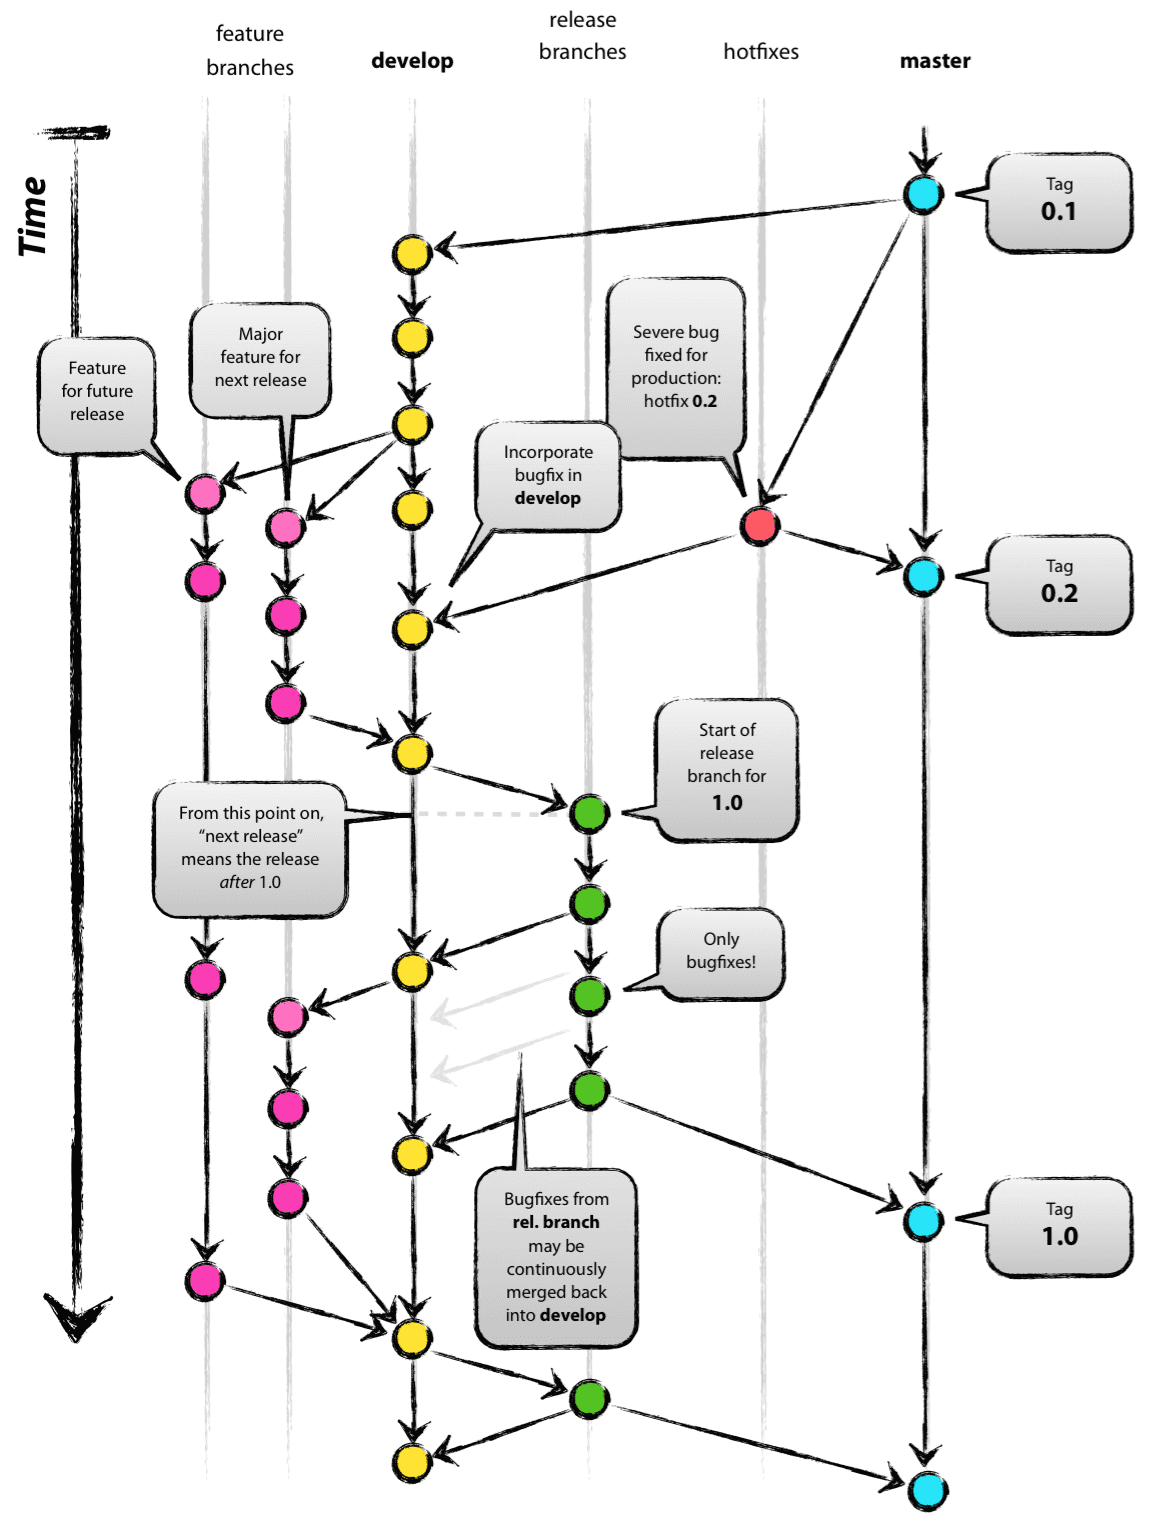
\includegraphics[scale=0.4]{images/git_branch_workflow.png}
		\caption{Git - Branch Workflow Model}
		\label{fig:git_branch_workflow_model}
	\end{figure}
	% subsection branching_model (end)
% section workflow (end)


\newpage \clearpage